\documentclass[a4paper,12pt]{report}

\usepackage{alltt, fancyvrb, url}
\usepackage{amssymb}
\usepackage{graphicx}
\usepackage{subfigure}
\usepackage{wrapfig}
% \usepackage{algorithm}% http://ctan.org/pkg/algorithms
% \usepackage[ruled, vlined]{algorithm2e}
% \usepackage{algorithm}
\usepackage[]{algorithm2e}
\usepackage{algorithmic}
\usepackage[utf8]{inputenc}
\usepackage{fontenc}
\usepackage{amsmath, stmaryrd, mathtools, algorithm}
\usepackage{amssymb}
%\usepackage{amsfonts}
\usepackage{float}
\usepackage{hyperref}
\usepackage{listings}
\usepackage{url}

\usepackage[english]{cleveref}

\usepackage[english]{babel}

\newtheorem{definition}{Definition}[section]
\newtheorem{theorem}{Theorem}[section]
\newtheorem{property}{Property}[section]
\newcommand{\R}{\mathbb{R}}
\newcommand{\Z}{\mathbb{Z}}
\newcommand{\F}{\mathbb{F}}
\newcommand{\dd}{\cdot}

\title{Introduction to Lattice-based Attacks\\``Cryptography''}
 
\author{Di Santi Giovanni}
\date{\today}

\begin{document}
 
\maketitle

\tableofcontents

\chapter{Introduction}

Lattices are powerful mathematical objects that can be used in computer science and mathematics to solves an extensive range of different problems.
In the recents years many post-quantum cryptographic protocols candidates involve the use of hard lattices problems,
for example the \textbf{Learning With Errors} \cite{LWE}.
Lattice constructions can also be used in cryptanalysis to break cryptographic schemes, typically using reduction
algorithms as \textbf{LLL} \cite{LLL}.

To introduce the mathematics of lattices a basic linear algebra background is needed, so the second chapter is a summary of the
basics properties needed to understand it. We used as main resource ``An Introduction to Mathematical Cryptography''\cite{mathcrypto14} to
explain them, but we also tried to give some geometrical intuition behind some operations.

Cryptographic protocol as \textbf{RSA} and \textbf{ECDSA} are considered secure, however there are various attacks against a
relaxed-model of each of them, i.e., What if we know some bits of the secret key? What if we know a part of the message before the encryption?
We present an introduction to the attacks which involves lattices against these protocols. The code used to confirm the correctness
of the attacks is available on the repository \cite{repo} and the main reference was
``Recovering cryptographic keys from partial information, by example''\cite{cryptoeprint:2020:1506}.

\chapter{Linear Algebra Background}

We'll start with some definitions and properties needed to understand the lattices, to move later on the mathematics behind them and some
hard problems related to it. At the end of the chapter the reader should be able to follow the math used in the other chapters.

\section{Vector Spaces}

\begin{definition}
    \textbf{Vector space}.
\end{definition}
A \textit{vector space} $V$ is a subset of $\R^{m}$ which is closed under finite vector addition and scalar multiplication, with the property that

\begin{center}
   $a_1v_1 + a_2v_2 \in V$ for all $v_1,v_2 \in V$ and all $a_1,a_2 \in \R$
\end{center}

\begin{definition}
    \textbf{Linear Combinations}
\end{definition}

Let $v_1,v_2,\ldots,v_k \in V$. A \textit{linear combination} of $v_1,v_2,\ldots,v_k \in V$ is any vector of the form:

\begin{center}
    $\alpha_1v_1 + \alpha_2v_2 + \cdots + \alpha_kv_k$ with $\alpha_1, \ldots, \alpha_k \in \R$
\end{center}

\begin{definition}
    \textbf{Linear Independece}
\end{definition}

A set of vectors $v_1,v_2,\ldots,v_k \in V$ is \textit{linearly independent} if the the only way to get

\begin{center}
    $a_1v_1 + a_2v_2 + \cdots + a_kv_k = 0$
\end{center}

is to have $a_1 = a_2 = \cdots = a_k = 0$.

\begin{definition}
    \textbf{Bases}
\end{definition}

Taken a set of linearly independent vectors $b = (v_1,\ldots,v_n) \in V$ we say that $b$ is a \textit{basis} of $V$ if $\forall w \in V$ we can write

\begin{center}
    $w = a_1v_1 + a_2v_2 + \cdots + a_nv_n$
\end{center}

\begin{definition}
    \textbf{Vector's length}
\end{definition}

The vector's length or \textit{Euclidean norm} of $v = (x_1, x_2, \ldots, x_m)$ is

\begin{center}
    $\lVert v \rVert = \sqrt{x_1^2 + x_2^2 + \cdots + x_m^2}$
\end{center}

\begin{definition}
    \textbf{Dot Product}
\end{definition}

Let $v, w \in V \subset \R^m$ and $v = (x_1, x_2, \ldots, x_m), w = (y_1, y_2, \ldots, y_m)$, the \textit{dot product} of $v$ and $m$ is

\begin{center}
    $v \dd m = x_1y_1 + x_2y_2 + \cdots + x_my_m$

    or

    $v \dd m = \lVert v \rVert \lVert w \rVert \cos{\theta}$
\end{center}

where $\theta$ is the angle between $v$ and $w$ if we place the starting points of the vectors at the origin $O$.

\begin{figure}[!b]
    \centering
    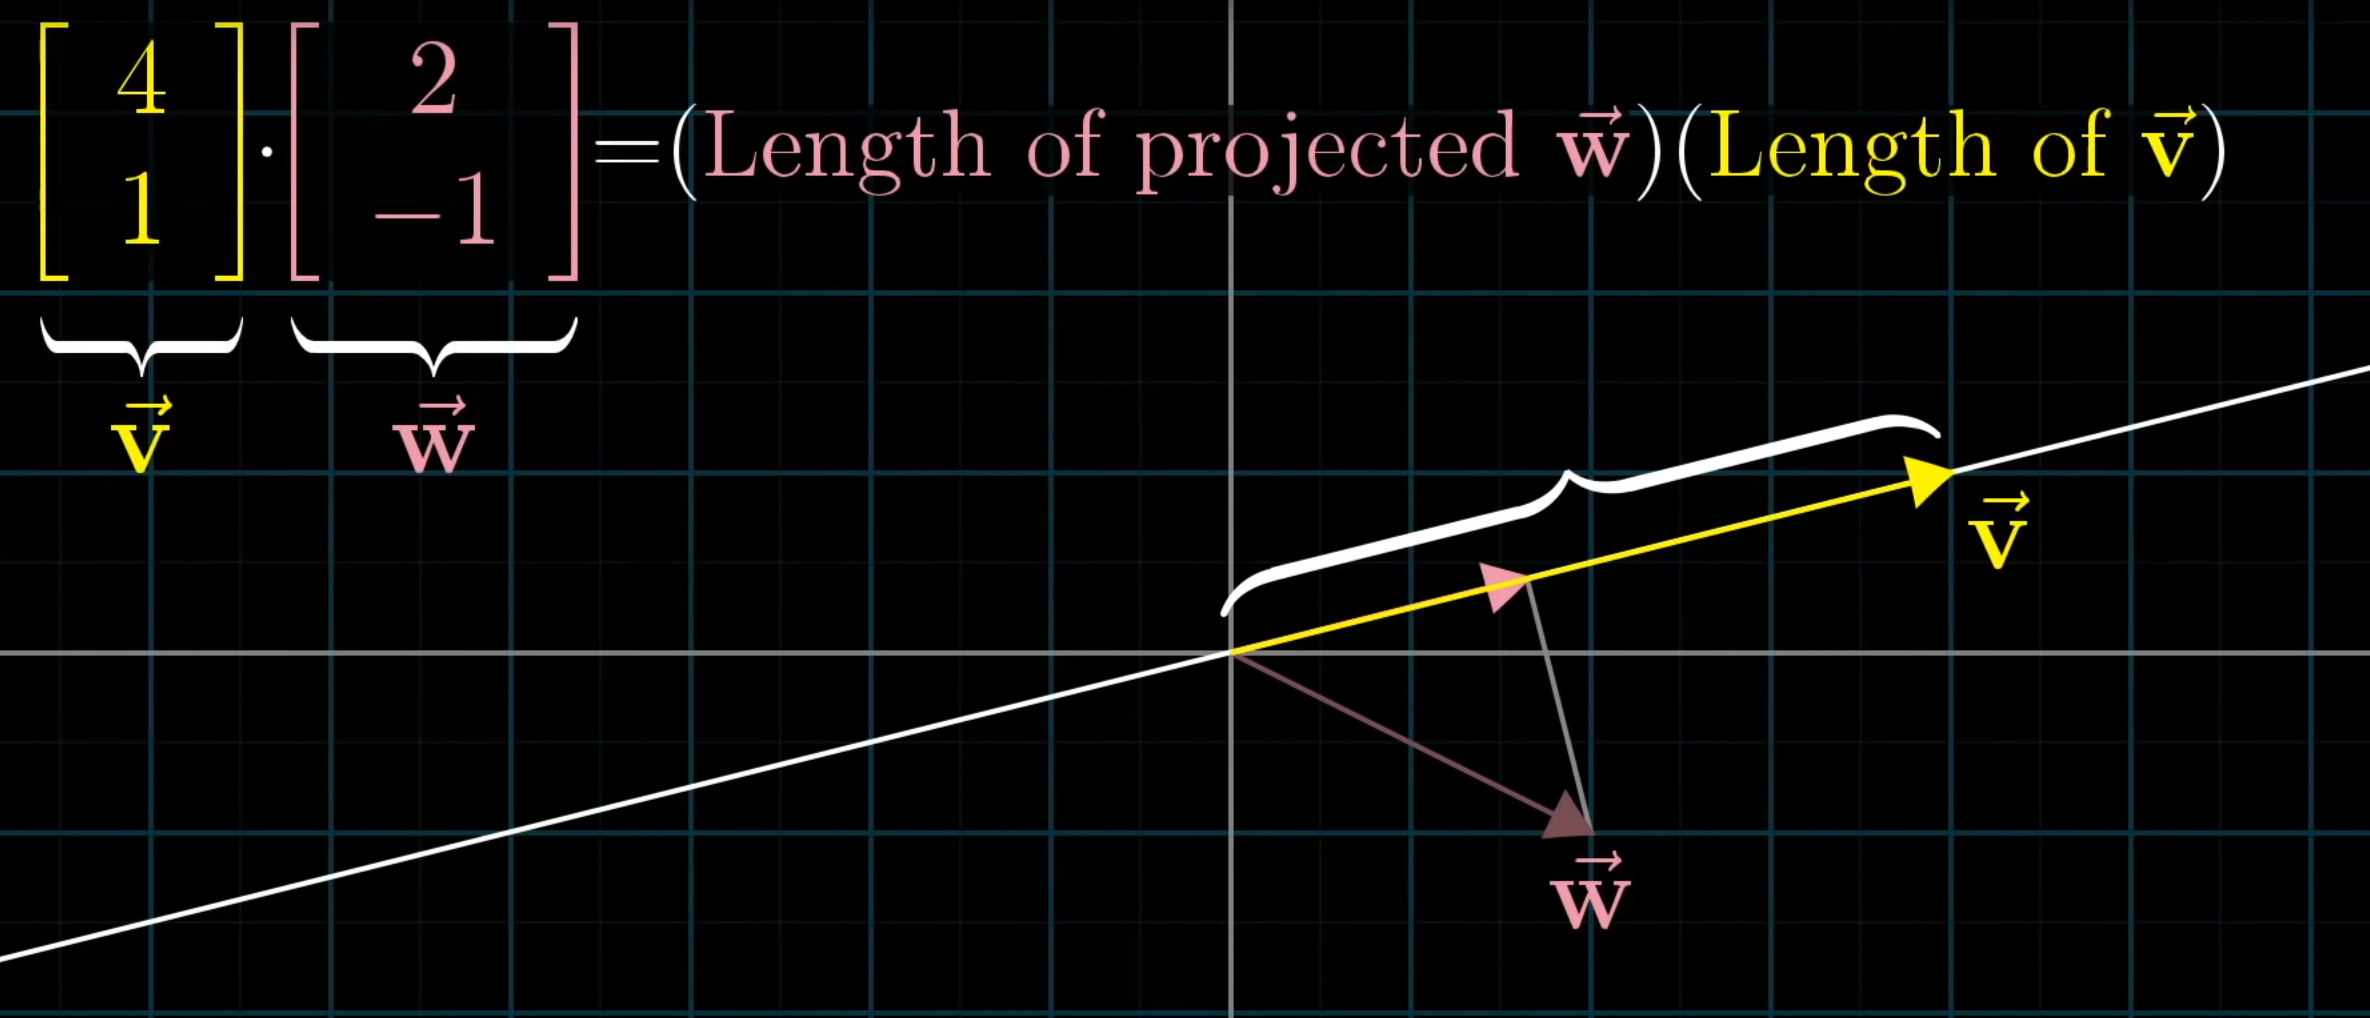
\includegraphics[scale=0.2]{./img/dot_product.png}
    \caption{Dot Product By 3Blue1Brown \cite{3b1b}}
    \label{fig:dot_product}
\end{figure}

Geometrically speaking $v \cdot m$ is the length of $w$ projected to $v$ multiplied by the length of $v$ as shown in \ref{fig:dot_product}

\begin{definition}
    \textbf{Ortoghonal Basis} 
\end{definition}

An \textit{ortoghonal basis} for a vector space $V$ is a basis $v_1, \ldots, v_m$ with the property that

\begin{center}
    $v_i \dd v_j = 0$ for all $i \neq j$
\end{center}

If $\lVert v_i \rVert = 1$ for all $i$ then the basis is \textit{orthonormal}.

\begin{algorithm}[H]
    \vspace*{5px}
    $v_1^* = v1$\;
    \\
    \For{$i \gets 2$ \KwTo $n$}{
        $\mu_{ij} = v_i \cdot v_j^* / \lVert v_j^* \rVert ^ 2$ for $1 \le j < i$ \;
        \\
        $v_i^* = v_i - \sum_{j=1}^{i-1} \mu_{ij}v_j^*$ \;
    }
    \caption{Gram-Schmidt Algorithm}
    \label{alg:gram_schmidt}
\end{algorithm}

Let $b = (v_1, \ldots, v_n)$, be a basis for a vector space $V \subset \R^m$. There is an algorithm to create an orthogonal basis
$b^* = (v_1^*,\ldots,v_n^*)$.
The two bases have the property that Span$\{v_1,\ldots,v_i\}$ = Span$\{v_1^*,\ldots,v_i^*\}$ for all $i = 1,2,\ldots,n$

\begin{figure}[htpb]
    \centering
    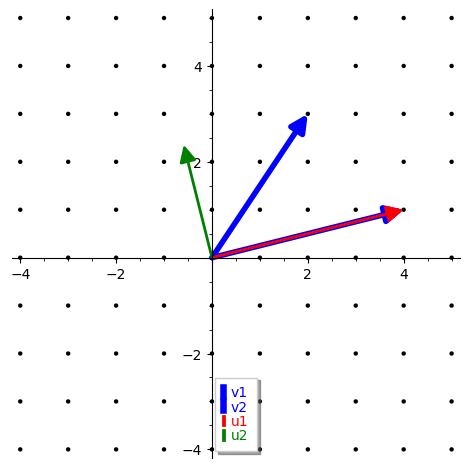
\includegraphics[width=0.5\textwidth]{./img/gram_schmidt.png}
    \caption{Gram Schmidt orthogonalization}
    \label{fig:gram_schmidt}
\end{figure}

If we take $v_1=(4, 1), v_2=(2, 3)$ as basis and apply gram schmidt we obtain $u_1=v_1=(4, 1), u_2=(-10/17, 40/17)$ as shown in \ref{fig:gram_schmidt}

\begin{definition}
    \textbf{Determinant}
\end{definition}

The \textit{determinant} of a square matrix is a function that satisfies the following properties:

\begin{enumerate}
    \item The determinant is linear in each row.
    \item The determinant reverses sign if two rows are interchanged.
    \item The determinant of the identity matrix is equal to 1.
\end{enumerate}

If the determinant of a matrix is $0$ then the matrix is called \textbf{singular} (without an inverse).\\

Grant Sanderson created fantastic animations to understand the geometrical intuition behind the \textit{determinant}\cite{determinant}.

\section{Lattices}

\begin{definition}
    \textbf{Lattice}
\end{definition}

Let $v_1,\ldots,v_n \in \R^m, m \ge n$ be linearly independent vectors. A \textit{Lattice} $L$ spanned by $\{v_1,\ldots,n_n\}$ is the set of 
all integer linear combinations of $v_1,\ldots,v_n$.

\begin{center}
    $L = \bigg\{\sum_{i=1}^{n} a_iv_i, a_i \in \Z \bigg\}$
\end{center}

If $v_i$ for every $i = 1,\ldots\,n$ has integer coordinates then the lattice is
called \textit{Integral Lattice}.

On the figure \ref{fig:lattice0} we show a lattice $L$ with bases $v=(3, 1)$ and $w=(-1, 1)$, and on \ref{fig:lattice1} the same lattice $L$ with
a different basis.

\begin{figure}[!bp]
    \begin{minipage}[b]{0.50\textwidth}
        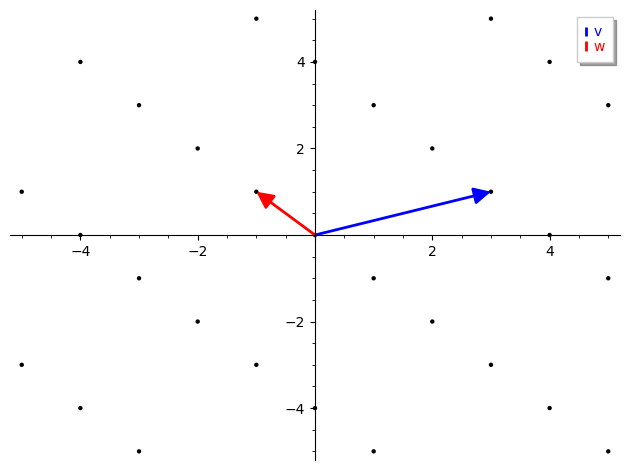
\includegraphics[width=\textwidth]{./img/lattice_b0.png}
        \caption{Lattice $L$ spanned by $v, w$}
        \label{fig:lattice0}
    \end{minipage}
    \hspace{\fill}
    \hspace{\fill}
    \hspace{\fill}
    \hspace{\fill}
    \hspace{\fill}
    \begin{minipage}[b]{0.50\textwidth}
        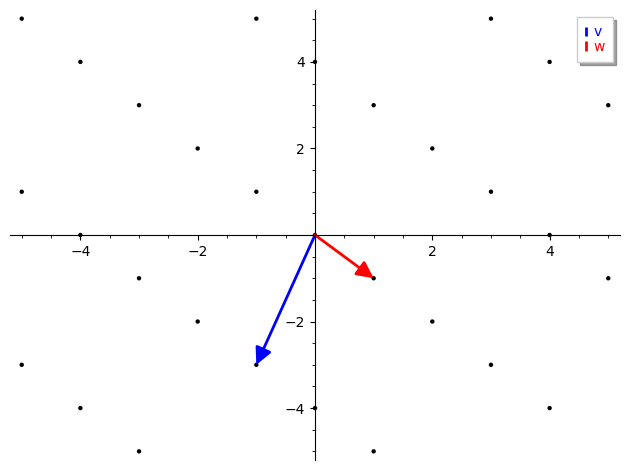
\includegraphics[width=\textwidth]{./img/lattice_b1.png}
        \caption{Lattice $L$ spanned by $v', w'$}
        \label{fig:lattice1}
    \end{minipage}
\end{figure}

\clearpage

\section{Lattice Problems}

\subsection{SVP}

\textbf{The Shortest Vector Problem} (\texttt{SVP}): \textit{Find a nonzero vector $v \in L$ that minimez the Euclidean norm $\lVert v \rVert$.}

Gauss's developed an algorithm to find an optimal basis for a two-dimensional lattice given an arbitrary basis. The output of the algorithm
gives the shortest nonzero vector in $L$ and in this way solves the \texttt{SVP}.

\begin{figure}[!b]
    \centering
    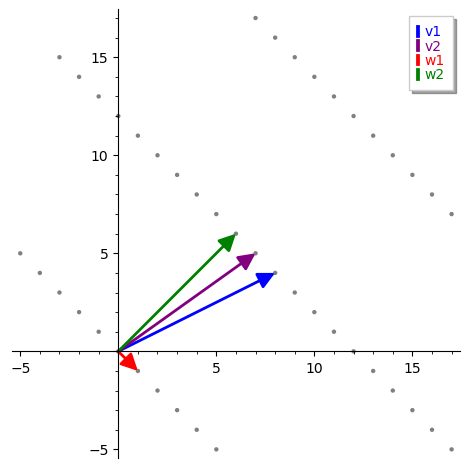
\includegraphics[width=0.6\textwidth]{./img/gauss_svp.png}
    \caption{Gauss reduction}
    \label{fig:gauss_svp}
\end{figure}

\begin{algorithm}[H]
    \vspace*{5px}
    \While{true}{
        \If{$\lVert v_2 \rVert < \lVert v_1 \rVert$}{
            swap $v_1, v_2$ \;
        }
        m = $\left \lfloor{(v_1 \cdot v_2) {\lVert v_1 \rVert}^{-2}} \right \rfloor$ \\
        \If{$m = 0$}{
            return $v_1, v_2$ \;
        }
        $v_2 = v_2 - mv_1$ \\
    }
    \caption{Gauss Basis Reduction}
\end{algorithm}

\textbf{Example}. Let $L$ a lattice spanned by $v_1 = (8, 4), v_2 = (7, 5)$, if we apply the gauss reduction algorithm we
obtain $w_1 = (1, -1), w_2 = (6, 6)$ \ref{fig:gauss_svp}. $w_1$ is the shortest nonzero vector in the lattice $L$.

The bigger the dimension of the lattice, the harder is the problem and there isn't a polynomial algorithm to solve it.

\subsection{CVP}

\textbf{The Closest Vector Problem} (\texttt{CVP}): \textit{Given a vector $t \in \R^m$ that is not in $L$, find the vector $v \in L$
    closest to $t$, in other words find a vector $v \in L$ that minimizes the Euclidean norm $\lVert t - v \rVert$.}

\begin{figure}[!ht]
    \centering
    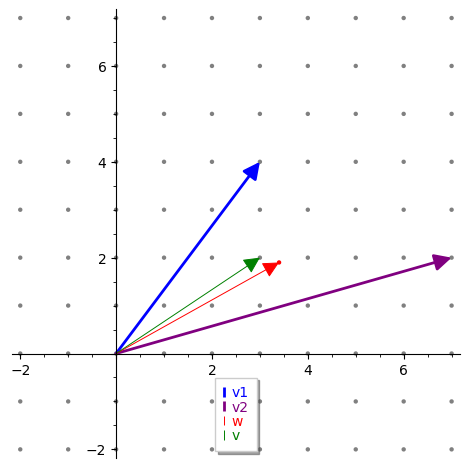
\includegraphics[width=0.6\textwidth]{./img/cvp.png}
    \caption{CVP}
    \label{fig:cvp}
\end{figure}

\textbf{Example}. Let $L$ a lattice spanned by $v_1 = (0, 1), v_2 = (2, 0)$, and a target vector $t = (2.3, 2.4)$. The closest vector
to $t$ in the lattice $L$ is $w = (2, 2)$.\\

Both \textbf{CVP} and \textbf{SVP} are $\mathcal{NP}$-hard problems, thus the complexity of the problem increments with the dimension
of the lattice. They can be used as primitive to create a trapdoor functions for a cryptographic scheme.

There are various algorithms that can output a solution under certain constraints for an approximation of both \textbf{SVP}
and \textbf{CVP}, for example \textbf{LLL}\cite{LLL} and \textbf{Babai's algorithm}\cite{babai} respectively.

\chapter{LLL}

\section{Introduction}

The \textbf{Lenstra-Lenstra-Lovász} \textit{LLL}\cite{LLL} or \textit{$L^3$} is a polynomial time algorithm to find a ``short'' basis of a lattice.

\begin{theorem}
    \textbf{LLL}
\end{theorem}

\textit{Let $L \in \Z^n$ be a lattice spanned by $B = \{v_1,\ldots,v_n\}$. The LLL algorithm outputs a reduced lattice
basis $\{w_1, \ldots, w_n\}$ with}

\begin{center}
    $\lVert w_i \rVert \le 2^{\frac{n(n-1)}{4(n-i+1)}} det(L)^{\frac{1}{n-i+1}}$ for $i=1,\ldots,n$
\end{center}

\textit{in time polynomial in n and in the bit-size of the entries of the basis matrix $B$}.\\

Basically the first vector of the new basis will be as short as possible, and the other will have increasing lengths. The new vectors
will be as orthogonal as possible to one another, i.e., the dot product $w_i \dd w_j$ will be close to zero.

\subsection*{Example}

For example we can take the following basis (the rows are the vector) that span
a lattice $L$.

\[
L = 
\begin{pmatrix}
    4 & 9 & 10\\
    2 & 1 & 30\\ 
    3 & 7 & 9
\end{pmatrix}
\] 

Applying the LLL algorithm we obtain

\[
LLL(L) = 
\begin{pmatrix}
    -1 & -2 & -1\\
     3 & -2 &  1\\
    -1 & -1 &  5
\end{pmatrix}
\] 

Where the first row is the shortest vector in the lattice $L$, and so solves the \textbf{SVP} problem.
For higher dimensions however the LLL algorithm outputs only an approximation for the \textbf{SVP} problem.

\section{Algorithm}

\begin{algorithm}[H]
    \vspace*{5px}
    Input basis ${v_1, \ldots, v_n}$ \; \\
    $k = 2$ \; \\
    $v_1* = v_1$ \; \\
    \While{$k \le n$}{
        \For{$j = k -1$ \KwTo $1$ step $-1$} {
            $v_k = v_k - \left\lfloor\mu_{k, j}\right\rceil \boldsymbol{v}_{j}$  [size-reduction] \;
        }
        \eIf{$\lVert v_k^* \rVert^2 \ge (\frac{3}{4} - \mu_{k, k-1}^2) \lVert v_{k-1}^2 \rVert$}{
            $k = k + 1$ \;  [Lovàsz-condition]
        }{
            Swap $v_{k-1}$ and $v_k$ [swap-step] \; \\
            $k = \max(k - 1, 2)$
        }
    }
    Note: At each step, $v_1^*, \ldots, v_k^*$ is the orthogonalized set of vectors
    obtained with the Gram-Schmidt \ref{alg:gram_schmidt}. \\
    \vspace*{5px}
    $\mu_{i,j}$ is the quantity $(v_i \cdots v_j^*) / \lVert v_j^* \rVert^2$. \\
    Output reduced basis ${v_1, \ldots, v_n}$
    \caption{LLL reduction algorithm}
\end{algorithm}

The running time of the algorithm is polynomial and executes the main loop no more than
$\mathcal{O}(n^2\log n + n^2\log M)$ steps, where $M = max \lVert v_i \rVert$. \\

Kelby Ludwig explains an intuition behind every step of the algorithm \cite{lllintuition}, and Oded Regev
gives a more rigorous explanation of the algorithm and the properties \cite{lllexplanation}.\\

Some applications of the algorithm are the following:

\begin{enumerate}
    \item Factoring polynomials over the integers. For example, given $x^2 - 1$ factor it into $x + 1$ and $x - 1$.
    \item Integer Programming. This is a well-known $\mathcal{NP}$-complete problem. Using \textbf{LLL}, one can obtain a polynomial time solution
          to integer programming with a fixed number of variables.
    \item Approximation to the \textbf{CVP} or \textbf{SVP}, as well as other lattice problems.
    \item Cryptanalysis (break cryptographic protocols).
\end{enumerate}

\chapter{RSA Cryptanalysis}

\section{RSA Introduction}

\subsection{Algorithm}

\textbf{RSA} is one of the earliest and most used asymmetric cryptosystem.
The usual step to generate a public/private key for \textbf{RSA} is the following

\begin{enumerate}
    \item Fix $e = 65537$ or $e = 3$ (public).
    \item Find two primes $p, q$ such that $p - 1$ and $q - 1$ are relatively prime to $e$, gcd$(e, p-1) = 1$ and gcd$(e, q-1) = 1$.
    \item Compute $N = p * q$ and $\phi(n) = (p-1) * (q-1)$
    \item Calculate $d$ (private) as the multiplicative inverse of $e$ modulo $\phi(n)$.
    \item $(N, e)$ is the public key, $(N, d)$ is the private key.
\end{enumerate}

To encrypt a message $m$ with \textbf{textbook RSA}

\begin{center}
    $c = m^e \mod N$
\end{center}

To decrypt a ciphertext $c$

\begin{center}
    $m = c^d \mod N$
\end{center}

\subsection{Security}

RSA relies on the hardness of factoring the modulo $N$, and we don't have a polynomial algorithm to factor it, so it's considered secure.
However, there are different attacks against textbook RSA or bad implementations:

\begin{itemize}
    \item If $m < N^{\frac{1}{e}}$, then $m^e < N$ and the modulo operation is not applied and we only need to find the $e$th root of $c$ over the
        integers to find $m$.
    \item If $q = p + x$ where $x$ is small enough than it's easy to recover the factors of $N$ computing $A = \sqrt{N}$ and compute
            $p = A - x$ for different value of $x$ until $N \mod p = 0$, then we have found $q = N / p$.
    \item It's possible to recover $d$ if it is too small (in practice could be used to accelerate decryption) using the Wiener's attack \cite{wiener}.
    \item Other attacks can be found on the excellent survey by Dan Boneh \cite{boneh99twentyyears}.
\end{itemize}

\section{Lattices against RSA}

We start introducing the main ideas of Coppersmith's attack \cite{coppersmith96} and the math behind it.
The attack can be used against \textbf{RSA} when a small $e$ is used, but also
to factorize the modulus if some bits of $p$ or $q$ are known. In 2017 the attack was used to exploit
\href{https://cve.mitre.org/cgi-bin/cvename.cgi?name=CVE-2017-15361}{CVE-2017-15361} also named \textbf{ROCA}
(Return Of Coppersmith's Attack) \cite{roca}.

\subsection{Mathematical introduction}

It's easy to find the roots of a univariate polynomial over the integers. Finding the roots of \textbf{modular} polynomial is hard, example:

\begin{center}
    $f(x) \equiv 0 \mod N$
\end{center}

Suppose $N$ is an \textbf{RSA} modulus, and we don't know the factorization of it. Let's have an univariate integer polynomial $f(x)$ with degree $n$

\begin{center}
    $f(x) = x^n + a_{n-1}x^{n-1} + a_{n-2}x^{n-2} + \cdots + a_1n + a_0$
\end{center}

Coppersmith showed how we can recover the value $x_0$ such that $f(x_0) \equiv 0 \mod N$, with $x_0 < N^{\frac{1}{n}}$ in polynomial time
using the following theorem

\clearpage

\begin{theorem}
    \textbf{Howgrave-Graham}
\end{theorem}

\textit{Let $g(x)$ be an univariate polynomial with n monomials and $m$ be a positive integer.
    If we have some restraint $X$ and the following equations hold}

\begin{center}
    \begin{eqnarray}
        g(x_0) \equiv 0 \mod N^m, |x_0| \le X \label{eq:bound} \\
         \lVert g(xX) \rVert < \frac{N^m}{\sqrt{n}} \label{eq:pol}
    \end{eqnarray}
\end{center}

\textit{Then $g(x_0) = 0$ holds over the integers.}

\vspace*{10px}

This theorem states that is possible to compute the root of $f(x) \mod N$ if we can find a polynomial $g(x)$ that share the same root but modulo $N^m$.
If \ref{eq:bound} and \ref{eq:pol} hold then we can simply compute the root of $g(x)$ over the integers to have the same root $x_0$
such that $f(x_0) \equiv 0 \mod N$.

Howgrave-Graham's idea is to find this polynomial $g$ by combining polynomials $p_i$ who also have $x_0$ as roots modulo $N^m$.

\vspace*{10px}

The \textbf{LLL} algorithm is fundamental because:

\begin{itemize}
    \item It only does \textbf{integer linear operations} on the basis vectors.
        In this way even if the basis is different it's only a linear combination of vector that still have $x_0$ as root
        modulo $N^m$.
    \item If we craft the lattice properly, the norm of the shortest vector on the reduced basis will satisfy \ref{eq:pol}.
        We know the length's bound of the shortest vector that LLL could find.
\end{itemize}

We can easily create polynomials $p_i$ ($g_{i,j}$ and $h_i$)  sharing the same root $x_0$ over $N^m$ of $f$ where $\delta$ is the degree of $f$:

\begin{center}
    \begin{eqnarray}
        g_{i,j}(x) &= x^j \cdot N^i \cdot f^{m-i}(x) \text{ for } i = 0,\hdots,m-1,\hspace{2mm} j=0,\hdots,\delta-1 \label{eq:create_pol} \\
        h_i(x) &= x^i \cdot f^m(x) \text{ for } i = 0,\hdots,t-1 
    \end{eqnarray}
\end{center}

Applying \textbf{LLL} to a lattice constructed by the coefficients of \ref{eq:create_pol} we'll find a short vector $v = g(xX)$ that will
satisfy \ref{eq:pol}. If we then take $g(x)$ we will be able to compute the root over the integer.

\subsection{Recover plaintext with known MSB bits of $m$}

We will use a simplified version of the Coppersmith's attack that works when the root is approximately less than $N^{\frac{1}{6}}$.

\textbf{Problem setup}. Let $N$ be an \textbf{RSA} modulus of $97$-bit:

\begin{center}
    $N=\texttt{0x1a34992f64135aedaa0fe2bfd}$ and $e = 3$.
\end{center}

Before the encryption the message $m$ is padded as

\[
    z = pad || m = \texttt{0xffffffffffffffffffffff} || m
\]

where $||$ is the concatenation.

The ciphertext is

\[
    c = z^e \mod N = \texttt{0x11701d5479bcdef207cba6937}
\]

Suppose that we don't know the factorization of $N$, and we would like to know the message $m$.
We know the padding and that the message $m$ is 2 bytes long, composed by only ascii letters, so $m < \texttt{0x7b7b}$.

\vspace*{10px}

Let's define

\[
    a = \texttt{0xffffffffffffffffffffff0000}
.\] 

which is the known padding string that got encrypted.

\vspace*{10px}

Thus, we have that $c = (a + m)^3 \mod N$, for an unkown small $m$.
We can define $f(x) = (a + x)^3 - c$, and setup the problem to find a small root $m$ such that $f(m) \equiv 0 \mod N$

\begin{align*}
    f(x) = x^3 + \texttt{0x17d7f55d0c9dc5851af54957c}x^2 + \texttt{0x3cf96fed2ea927527a2ed329}x\\
    + \texttt{0x32882e547964b3bcf75d315e}
\end{align*}

\vspace*{10px}

\textbf{Lattice contruction}. Let the coefficients of $f$ be $f(x) = x^3 + f_2x^2 + f_1x + f_0$
and $X = \texttt{0x7b7b}$ be the upper bound of the size of the root $m$. We can construct the matrix

\[
B = 
\label{mat:lattice_rsa}
\begin{pmatrix}
    X^3 & f_2X^2 & f_1X & f_0 \\
    0 & NX^2 & 0 & 0 \\
    0 & 0 & NX & 0 \\
    0 & 0 & 0 & N
\end{pmatrix}
\] 

The rows of the matrix correspond to the coefficient vectors of the polynomials $f(x), Nx^2, Nx$ and $N$, furthermore we know
that each polynomial will be 0 modulo $N$ if evaluated at $x = m$.
We applied Howgrave-Graham with $m=1$ (the $N^m$ parameter not the message).\\
With this lattice construction every vector is of the form $v = (v_3X^3, v_2X^2, v_1X, v_0)$, because any
integer linear combination of the vector of the lattice will keep the bound $X^i$ for $i=\dim(B)-1,..,0$.

\textbf{Apply LLL}. We then apply LLL to find the shortest vector of the reduced basis:

\[
    \begin{split}
    v = (-\texttt{0xd55d67baf71d}X^3, \texttt{0x3cf3cca3200a58bf}X^2, \\
    \texttt{0x3854d44211e80f248449}X, -\texttt{0xec93bf51cf766f7b9f1e5e6})
    \end{split}
\]

We can construct the polynomial $g$ using the coefficients of $v$

\[
    \begin{split}
        g(x) = -\texttt{0xd55d67baf71d}x^3 +  \texttt{0x3cf3cca3200a58bf}x^2 \\
        \texttt{0x3854d44211e80f248449}x -\texttt{0xec93bf51cf766f7b9f1e5e6}
    \end{split}
\]

We know that

\[
    g(x_0) \equiv 0 \mod N, |x_0| \le X
\]

What we need to prove is that

\[
    \lVert g(xX) \rVert \le \frac{N}{\sqrt{n}}
\] 

In this example, det $B = X^6N^3$, and LLL will find a short vector with $\lVert v \rVert \le 2^{\frac{n(n-1)}{4(n)}} (\det B)^{\frac{1}{n}}$.
If we ignore the $2^{\frac{3}{4}}$ factor (remember that $n = 4$), then we need to satisfy

\[
    g(m) \le \lVert v \rVert \le (\det B)^{\frac{1}{4}} < \frac{N}{\sqrt{4}}
\] 

\vspace*{10px}

We have $(\det B)^{\frac{1}{4}} = (X^6N^3)^{\frac{1}{4}} < \frac{N}{\sqrt{4}}$, if we solve for $X$ this will be satisfied when
$X < (\frac{N}{16})^{\frac{1}{6}}$. We can consider the $\sqrt{4}$ an error term to have $X < N^{\frac{1}{6}}$.
With the numbers we have this inequality is verified, however even if the bound of the shortest vector is larger we still have some possibilities to
find the correct root.

Computing the root of $g(x)$ over the integers we obtain $m = \texttt{0x4142} = $ ``AB'' which is the correct result.\\

This specific lattice works to find roots up to size $N^{\frac{1}{6}}$, so the same construction will work if we want to find

\begin{itemize}
    \item $\approx$ 170 unkown bits of message from an RSA 1024-bit modulus
    \item $\approx$ 341 unkown bits of message from an RSA 2048-bit modulus
    \item $\approx$ 683 unkown bits of message from an RSA 4096-bit modulus
\end{itemize}

To compute bigger root a bigger lattice with more polynomials generated with \ref{eq:create_pol} is needed,
this method is better described in \cite{may2011} and a detailed implementation in sagemath by David Wong is available \cite{wong2015}.

\subsection{Factorize modulus with known MSB bits of $p$}

Lattices can also be used to factor a modulus $N$ knowing the most significant bits of one of the factor.
Let $a = 2^lb$ where $b$ are the bits known of $p$, then $p = a + r$ for some small value of $r$.
We can rewrite the problem to find the root $r$ of $f(x) = a + x \mod p$ such that $f(r) = p \equiv 0 \mod p$.
Suppose that we know the bound of $r$ such that $|r| < X$ for some bound $X$.

We can construct the following lattices

\[
    B = 
    \begin{pmatrix}
        X^2 & Xa & 0 \\
        0 & X & a \\
        0 & 0 & N
    \end{pmatrix} 
\]

\vspace*{10px}

Notice that the rows correspond to the polynomials $x(x + a)$, $(x + a)$, $N$ and that each of these polynomials will
be $0 \mod p$ when $x = r$. As before \ref{mat:lattice_rsa}, every polynomial is scaled by $X$ which is the upperbound.

We need to verify that the shortest vector that we can find with \textbf{LLL} will be less than $p$ because if $g(x) < p$,
then by construction we can compute $g(r) = 0$ over the integers.
In this case we have

\[
    (detB)^{\frac{1}{\dim L}} = (X^3N)^{\frac{1}{3}} < p
\]

Solving for $X$ we obtain $X < p^{\frac{1}{3}}$, so this method works for every $|r| < p^{\frac{1}{3}}$.

To find $r$ we just need to apply \textbf{LLL} and take the first vector (shortest) that will be of the form $v = (v_2X^2, v_1X, v_0)$.

The last step is to construct $g(x) = v_2x^2 + v_1x + v_0$ (just divides every coefficient by $X^i$)
and computes the roots over the integers to find $r$. We implemented the attack against a modulus
of \textbf{RSA}-$1024$ knowing the $160$ most significant bits of $p$. The attack can be expanded
until $X < p^{\frac{1}{2}}$ with a bigger lattice.

\subsection{Real world case study: ROCA}

\textbf{ROCA}\cite{roca} is a vulnerability discovered in 2017 in a software library \textit{RSALib} in the generation
of the public modulus for \textbf{RSA}. The attack is believed to affect millions of smart cards. The vulnerbality
resides in the generation of prime numbers, since embedded devices don't have lots of computational resources a fast way
was needed. Every prime generated has the following structure:

\[
    p = kM + (g^a \mod M)
    \label{eq:roca}
\]

Where $k, a$ are random values different for every prime (unkown), $g = 65537$ and $M$ it's a \textit{primorial} number.
A \textit{primorial} number $M$ is the product of the first $n$ successive primes 

\[
    M = P_n\# = \prod_{i=1}^{n} P_i
\]

where $n$ is related to key size. In the case of \textit{RSALib} the primorial number used had similar dimension to $p$,
and the value $a, k$ didn't have much entropy. The modulus is

\[
    N = (kM + g^{a}\mod M)(lM + g^{b}\mod M)
\]

for $a, b, k, l \in \Z$. It's equivalent to

\[
    N \equiv g^{a + b} \equiv g^{c} \mod M
\]

for some $c \in \Z$ since all the multiples of $kM$ or $lM$ are $0 \mod M$.

It's possible to compute the discrete logarithm of $g^c \mod M$ since the size of $|M|$ is smooth with
Pohlig-Hellman algorithm \cite{pohlig}. With $c$ we can set the bound to the value of $a$ since

\[
    \frac{c}{2} \le a \le \frac{c + ord}{2}
\]

where $ord$ is the multiplicative order of the generator $g \in Z_M$.

Once we know the bound of $a$ we can try to find the value of $k$ with the Coppersmith's method \cite{coppersmith96} for every possible $a$.

The concept of the algorithm is the following:

\begin{algorithm}[H]
    \vspace*{5px}
    \textbf{Input: } $N, M, g, ord, X$ \; \\
    $c = \log_{g}N \mod M$ \;\\
    \For{$a \gets (\frac{c}{2}, \frac{c + ord}{2})$}{
        \vspace*{5px}
        $f(x) = xM + (g^a \mod M)$ \; \\
        $g(x) = \frac{1}{M}f(x)$ [make monic, the roots are the same] \; \\
        $k = $ coppersmith($g(x), N, X$) [find k] \; \\ 
        $p = kM + (g^a \mod M)$  [candidate] \; \\
        \If{$N \mod p = 0$}{
            return $p$ \;
        }
    }
    \caption{Exploit idea}
\end{algorithm}

In practice however the bound of $a$ is too big, so the authors found a way to move the same problem to a smaller $M'$ since the
bitsize of $M$ are more than sufficient for making the attack works with Coppersmith's algorithm. Their optimization
find a new $M'$ such that

\begin{itemize}
    \item $(p, q)$ are still of the form \ref{eq:roca}, so $M'$ must be a divisor of $M$.
    \item Coppersmith's algorithm will find $k'$ for the correct guess of $a'$.
    \item Find a small order of $g \in \Z_M'$ to make $a'$ smaller.
\end{itemize}

We were able to reproduce the attack in sagemath against \textbf{RSA}-$512$, and we used as $M'$ the value
that Bruno Produit \cite{rocaopt} made available in his thesis and David Wong's implementation of Coppersmith's attack \cite{wong2015}.

\chapter{ECDSA Cryptanalysis}

\section{ECDSA Introduction}

\subsection{Algorithm}

\textbf{ECDSA} is a variant of the Digital Signature Algorithm (\textbf{DSA}) which uses elliptic curve cryptography.
There are 3 public parameters:

\begin{itemize}
    \item The elliptic curve \textbf{$E$}.
    \item The generator point \textbf{$G$}.
    \item The generator's order \textbf{$n$}.
\end{itemize}

We also need to create a private key $d \in [1, n-1]$ and public key $Q = dG$. To \textbf{sign} a message $m$:

\begin{enumerate}
    \item Compute $h = $ MSB(HASH$(m))$ where HASH is a cryptographic hash function, for example SHA-256, and MSB take the $n$ most significant bits.
    \item Select a random integer $k \in [1, n-1]$ (nonce).
    \item Calculate $P = kG = (x_1, y_1)$ and set $r = (x_1)$ if $x_1 \neq 0$, otherwise repeat the steps.
    \item Compute $s = k^{-1}(h + dr) \mod n$, if $s = 0$ repeat the steps.
    \item The signature is composed by $(r, s)$.
\end{enumerate}

\clearpage

To \textbf{verify} the signature:

\begin{enumerate}
    \item Compute $h = $ HASH$(m)$.
    \item Calculate $u_1 = hs^{-1} \mod n$ and $u_2 = rs^{-1} \mod n$.
    \item Compute $P = u_1G + u_2Q = (x_1, y_1)$, if $P = O$ the signature is invalid.
    \item If $r \equiv x_1 \mod n$ then the signature is valid.
\end{enumerate}

\subsection{Security}

The security of \textbf{ECDSA} depends on the discrete logarithm problem.
Given the points $Q, G$ such that $Q = k*G$ it's considered an hard problem to find $k$.
However, as RSA, there are lots of implementation attacks

\begin{itemize}
    \item If the same $k$ is used to generate two different signatures it's possible to recover the secret key $d$. This was a real bug 
        discovered in the Playstation 3.
    \item It's possible to recover $d$ if the parameter $k$ is not generated with a cryptographically secure pseudo random generator.
    \item If the elliptic curve used is not standardized (custom) then it's possible that the discrete logarithm is easily solvable
        \cite{giuliani99attackson}, \cite{mov} \cite{smartass}.
\end{itemize}

\section{Lattices against ECDSA}

The lattice-based attacks presented here are based on the \textit{HNP (Hidden Number Problem)} introduced
by Boneh and Venkatesan \cite{hnp} that was in a second moment generalized to prove that the most significant bits
of $k$ can potentially leak the entire nonce \cite{ecdsa_nonce}.
In 2020 a group of researcher were able to leak the MSBs of \textit{DH} and \textit{DHE} secrets in \textbf{TLS $\le$ 1.2}
and used a similar lattice constructions as the one we will describe to solve the \textit{HNP}
and thus break the protocol \cite{cryptoeprint:2020:1151} (Raccoon Attack).

\subsection{Recover $d$ from a pair of signatures with small $k_1, k_2$}

\textbf{Problem setup}.
Let $p = \texttt{0xffffffffffffd21f}$ and let $E: y^2 = x^3 + 3$ be an elliptic curve over $\F_p$ with the generator
$G = (\texttt{0xcc3b3d1a0c4938ef}, \\ \texttt{0x4ab35ff66f8194fa})$ of order $n = \texttt{0xfffffffefa23f437}$.

\clearpage

We have two signature:

\[
    \begin{array}{c}
        (r_1, s_1) = (\texttt{0x269fa43451c5ff3c}, \texttt{0x1184ec0a74d4be7c}) \\
        \text{and hash } h_1 = \texttt{0xb526aef1a341cfe6}
    \end{array}
\]

\[
    \begin{array}{c}
        (r_2, s_2) = (\texttt{0xf77cda14f5bf50a2}, \texttt{0xcd1143ccc1516b02}) \\ 
        \text{and hash } h_2 = \texttt{0x84768ddee659efea}
    \end{array}
\]

And we know that both of these signatures use 32-bit nonce $k$, note that $n$ is a 64-bit number. We can set up the problem as a system of equation

\[
    \begin{array}{c}
        s_1 \equiv \displaystyle\frac{h_1 + dr_1}{k_1} \mod n \\ \\ 
        s_2 \equiv \displaystyle\frac{h_2 + dr_2}{k_2} \mod n
    \end{array}
\]

We don't know $d, k_1, k_2$, but we can write 

\[
    d = \displaystyle\frac{s_1k_1 - h_1}{r_1}
\]

and rewrite the equation in

\[
    k_1 - s_1^{-1}s_2r_1^{-1}k_2 + s_1^{-1}r_1h_2r_2^{-1} - s_1^{-1}h_1 \equiv 0 \mod n
\]

To simplify the equation we write $t = - s_1^{-1}s_2r_1^{-1}k_2$ and $u = s_1^{-1}r_1h_2r_2^{-1} - s_1^{-1}h_1$. In this way we have

\[
    \begin{array}{c}
        k_1 + tk_2 + u \equiv 0 \mod n \\
        \text{or} \\
        -k_1 = tk_2 + u - xn \text{   for some $x$}
    \end{array}
\]

We know that $|k_1|, |k_2| < K = 2^{32}$.

\vspace*{10px}

\textbf{Lattice construction}. We construct the lattice $B = (b_0, b_1, b_2)$:

\[
    B = 
    \begin{pmatrix}
        n & 0 & 0 \\
        t & 1 & 0 \\
        u & 0 & K
    \end{pmatrix}
\]

Note that the vector $v = (-k_1, k_2, K)$ is in the lattice because

\[
    v = -xb_0 + k_2b_1 + b_2 = (-xn + tk_2 + u = -k_1, k_2, K)
\]

for some $x, k_2 \in Z$.

\vspace*{10px}

Can we prove that $v$ is a short vector that we can find with LLL?

We have 

\begin{center}
    $\lVert v \rVert = \sqrt{k_1^2 + k_2^2 + K^2} \le \sqrt{3K^2} = \sqrt{3}K $
\end{center}

And we expect the shortest vector to have length

\[
    \begin{array}{c}
        \approx 2^{\frac{1}{2}}(\det B)^{\frac{1}{3}} \\
        \approx 2^{\frac{1}{2}}(nK)^{\frac{1}{3}}
    \end{array}
\]

So we want that 

\begin{center}
    $\lVert v \rVert \le \sqrt{3}K < \sqrt{2}(nK)^{\frac{1}{3}}$
\end{center}

And if we remove the smaller terms this will be satisfied when $K < (nK)^{\frac{1}{3}}$ or $K < \sqrt{n}$.

In this case if we apply LLL in the second row we obtain:

\begin{center}
    $v = (-k_1, k_2, K) = (\texttt{-0x50a65330, 0x1f5b977a, 0x100000000})$
\end{center}

To retrieve $d$ we just need to compute 

\[
    d = r_1^{-1}(k_1s_1 - h_1) = \texttt{0xf00e5fb275bfd304}
\]

%Boneh-Venkatesan1996_Chapter_HardnessOfComputingTheMostSign-1.pdf, HPL-1999-90-1.pdf, https://www.researchgate.net/publication/2406712_The_Insecurity_of_the_Elliptic_Curve_Digital_Signature_Algorithm_with_Partially_Known_Nonces

\subsection{Recover $d$ from many signatures with small $k_i$}

Suppose we have many signatures $(r_1, s_1), \ldots, (r_m, s_m)$ with message hashes $h_1, \ldots, h_m$. We can write the equivalence
$s_i \equiv k_i^{-1}(h_i +  dr_i) \mod n$ for $i = 1,\ldots,m$ and we can remove $d$ as before to get

\[
\begin{array}{c}
    k_1 + t_1k_m + u_1 \equiv 0 \mod n \\
    k_2 + t_2k_m + u_2 \equiv 0 \mod n \\
    \vdots \\
    k_{m-1} + t_{m-1}k_m + u_{m-1} \equiv 0 \mod n
\end{array}
\]

\vspace*{10px}

And create the lattice $B$ as

\[
    B = 
    \begin{pmatrix}
     n &  \\
     & n \\
     & & \ddots \\
     & & & n \\
     t_1 & t_2 & \cdots & t_{m-1} & 1 & 0 \\
     u_1 & u_2 & \cdots & u_{m-1} & 0 & K
     \label{eq:lattice_ecdsa}
    \end{pmatrix}
\]

\vspace*{10px}

Same as before this lattice contains $v = (-k_1, -k_2, \ldots, k_m, K)$ that can be found using LLL.

\subsection{Recover $d$ knowing MSB bits of each $k_i$}

What if we know the firsts MSB bits of each $k_i$?

Well, we can write $k_i = (a_i + b_i)$, where $a_i$ is the known part and $b_i$ is the unkown part that satisfies $|b_i| < K$. If we plug these values
into the equivalence we obtain

\[
    \begin{array}{c}
        k_i + t_ik_m + u_i \equiv 0 \mod n \\
        (a_i + b_i) + t_i(a_m + b_m) + u_i \equiv 0 \mod n \\
        b_i + t_ib_m + a_i + t_ia_m + u_i \equiv 0 \mod n \\
    \end{array}
\]

And we can set $u_i' = a_i + t_ia_m + u_i$ to be the value inside the lattice \ref{eq:lattice_ecdsa} instead of $u_i$. In this way the vector

\begin{center}
    $v = (-b_1, -b_2, \ldots, b_m, K)$
\end{center}

is in the lattice and could be found using LLL. To recover the original $(k_1, \ldots, k_m)$ we must add to $v$ the vector $w = (a_1, \ldots, a_m)$.

Without any optimization we were able to recover the nonces with the $8$ MSB bits known on the curve \texttt{secp256r1} given $100$ signatures 
and with a probability bigger than $50\%$ with $7$ MSB bits known.

It's possible to optimize the attack to recover the nonces with less known bits as shown in the results obtained by
Albrecht and Heninger \cite{ecdsa_result}.

\chapter*{Conclusion}

The results obtained from the implementation of the attacks are satisfactory and can be used against real world practical cases.
There is a fair amount of probability and heuristic to make the attacks works that isn't discussed in detail.
As with other branch of mathematics not all theorems and properties are proved to be useful the moment they were first introduced
but can become useful years later as the hidden number problem that become crucial for the Raccoon Attack.
The study on how to exploit side-channel attacks (ex. knowing some bits of $p$ in \textbf{RSA}) has been proven useful
with \textbf{ROCA}.
The most used cryptographic protocol used has been proved secure but it's very easy to implement them wrong and side-channel
vulnerabilities can heavily compromise the security of the protocols.

\bibliographystyle{plain}

\bibliography{lattice_based_attacks}

\end{document}

